\documentclass[12pt, english]{article}
\usepackage{pgfplots}
\usepackage{tikz}
\usepackage{comment}
\usepackage{polynom}
\usepackage{ulem}
\usepackage{xcolor}
\usepackage{varwidth}
\usepackage{amsmath, amsthm, amssymb}
\usepackage[makeroom]{cancel}
\usepackage{relsize}
\usepackage{gensymb}
\usepackage[top=1in,bottom=1in,right=1in,left=1in]{geometry}
\usepackage{tkz-euclide}
\usetkzobj{all}
\usetikzlibrary{arrows}
\title{Reference Book}
\author{Zane Helton}
\date{} % To make the properties fit on the same page as the plot
\begin{comment}
\pgfplotsset {
	after end axis/.code = {
		\node[style={fill=blue,circle,inner sep=0pt,minimum size=4pt},pin={[text=blue,text width=3cm,pin edge={black,thick}]20-45:{\small{'12 MTT\\65nm CMOS}}}] at (axis cs:5, 5) { };
	}
}			
\end{comment}

\newcommand{\specialcell}[2][c]{%
  \begin{tabular}[#1]{@{}c@{}}#2\end{tabular}}

 \newdimen\tcolw \tcolw=2.5em % the column width
\edef\ecatcode{\catcode`&=\the\catcode`&\relax}\catcode`&=4
\def\sgchart#1#2{\vbox{\offinterlineskip\halign{\hfil##\quad&##\hfil\crcr\sgchartA#2,:,%
   \omit\sgchartR&\kern.2pt\sgchartS{.5\tcolw}\relax\sgchartE#1,\relax,%
   \sgchartS{.5\tcolw}\relax\cr
   \noalign{\kern2pt}&\def~{}\kern.5\tcolw\sgchartD#1,\relax,\cr}}}
\def\sgchartA#1:#2,{\cr\ifx,#1,\else $#1$&\sgchartB#2{}\expandafter\sgchartA\fi}
\def\sgchartB#1{\hbox to\tcolw{\hss$#1$\hss}\sgchartC}
\def\sgchartC#1{\ifx,#1,\else
   \strut\vrule\kern-.4pt\hbox to\tcolw{\hss$#1$\hss}\expandafter\sgchartC\fi}
\def\sgchartD#1#2,{\ifx\relax#1\else\hbox to\tcolw{\hss$#1#2$\hss}\expandafter\sgchartD\fi}
\def\sgchartE#1#2,{\ifx\relax#1\else
    \ifx~#1\sgchartS\tcolw\circ \else\sgchartS\tcolw\bullet\fi \expandafter\sgchartE\fi}
\def\sgchartR{\leaders\vrule height2.8pt depth-2.4pt\hfil}
\def\sgchartS#1#2{\hbox to#1{\kern-.2pt\sgchartR \ifx\relax#2\else
   \kern-.7pt$#2$\kern-.7pt\sgchartR\fi\kern-.2pt}}
\ecatcode
 
\begin{document}
	\maketitle
	\pagebreak
	\section{12 Basic Functions}
	\subsection{Linear Function}
	\begin{center}
		\begin{tikzpicture}		\end{tikzpicture}
	
		\subsection*{\underline{Properties}}
		\begin{tabular}{|c|c|}
			\hline
				Domain & $(-\infty, \infty)$\\
				Range & $(-\infty, \infty)$\\
			\hline
				Continuous & Yes\\
			\hline
				Symmetry & Odd\\
			\hline
				Increasing & $(-\infty, \infty)$\\
			\hline
				Bounded & No\\
			\hline
				Extrema & None\\
			\hline
				Asymptotes & None\\
			\hline
				Limits & \specialcell{$\lim_{x \to -\infty} f(x) = -\infty$\\
									  $\lim_{x \to \infty} f(x) = \infty$}\\
			\hline
		\end{tabular}
	\end{center}
	
	\subsection{Quadratic Function}
	\begin{center}
		\begin{tikzpicture}		\end{tikzpicture}
	
		\subsection*{\underline{Properties}}
		\begin{tabular}{|c|c|}
			\hline
				Domain & $(-\infty, \infty)$\\
				Range & $(0, \infty)$\\
			\hline
				Continuous & Yes\\
			\hline
				Symmetry & Even\\
			\hline
				Increasing & $[0, \infty)$\\
				Decreasing & $(-\infty, 0]$\\
			\hline
				Bounded & Below\\
			\hline
				Extrema & Minimum: $(0, 0)$\\
			\hline
				Asymptotes & None\\
			\hline
				Limits & \specialcell{$\lim_{x \to -\infty} f(x) = \infty$\\
									  $\lim_{x \to \infty} f(x) = \infty$}\\
			\hline
		\end{tabular}
	\end{center}
	
	\subsection{Cubic Function}
	\begin{center}
		\begin{tikzpicture}		\end{tikzpicture}
	
		\subsection*{\underline{Properties}}
		\begin{tabular}{|c|c|}
			\hline
				Domain & $(-\infty, \infty)$\\
				Range & $(-\infty, \infty)$\\
			\hline
				Continuous & Yes\\
			\hline
				Symmetry & Odd\\
			\hline
				Increasing & $(-\infty, \infty)$\\
			\hline
				Bounded & No\\
			\hline
				Extrema & None\\
			\hline
				Asymptotes & None\\
			\hline
				Limits & \specialcell{$\lim_{x \to -\infty} f(x) = -\infty$\\
									  $\lim_{x \to \infty} f(x) = \infty$}\\
			\hline
		\end{tabular}
	\end{center}
	
	\subsection{Reciprocal Function}
	\begin{center}
		\begin{tikzpicture}		\end{tikzpicture}
	
		\subsection*{\underline{Properties}}
		\begin{tabular}{|c|c|}
			\hline
				Domain & $(-\infty, 0)\bigcup(0, \infty)$\\
				Range & $(-\infty, 0)\bigcup(0, \infty)$\\
			\hline
				Continuous & Infinite discontinuity\\
			\hline
				Symmetry & Odd\\
			\hline
				Decreasing & $(-\infty, 0)\bigcup(0, \infty)$\\
			\hline
				Bounded & No\\
			\hline
				Extrema & None\\
			\hline
				Asymptotes & \specialcell{$y = 0$\\$x = 0$}\\
			\hline
				Limits & \specialcell{$\lim_{x \to -\infty} f(x) = 0$\\
									  $\lim_{x \to \infty} f(x) = 0$}\\
			\hline
		\end{tabular}
	\end{center}
	
	\subsection{Square Root Function}
	\begin{center}
		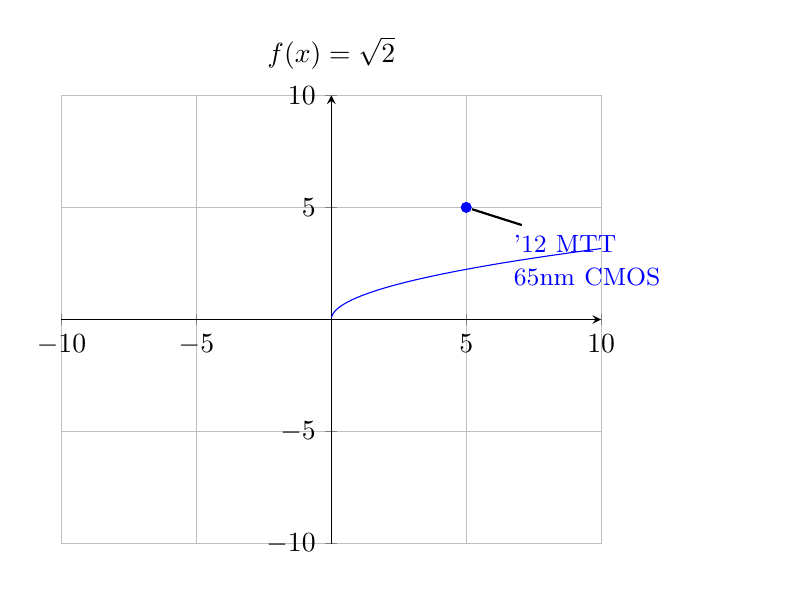
\begin{tikzpicture}
			\begin{axis} [
				axis lines = center,
				xmax = 10,
				xmin = -10,
				ymax = 10,
				ymin = -10,
				grid = major,
				title = {$f(x) = \sqrt2$},
				samples = 1000
			]
				\addplot[smooth, no marks, blue, domain = -10:10] {x^(1/2)};
			\end{axis}
		\end{tikzpicture}
	
		\subsection*{\underline{Properties}}
		\begin{tabular}{|c|c|}
			\hline
				Domain & $[0, \infty)$\\
				Range & $[0, \infty)$\\
			\hline
				Continuous & Yes\\
			\hline
				Symmetry & None\\
			\hline
				Increasing & $[0, \infty)$\\
			\hline
				Bounded & No\\
			\hline
				Extrema & Minimum: $(0, 0)$\\
			\hline
				Asymptotes & None\\
			\hline
				Limits & \specialcell{$\lim_{x \to -\infty} f(x) = DNE$\\
									  $\lim_{x \to \infty} f(x) = \infty$}\\
			\hline
		\end{tabular}
	\end{center}
	
	\subsection{Exponential Function}
	\begin{center}
		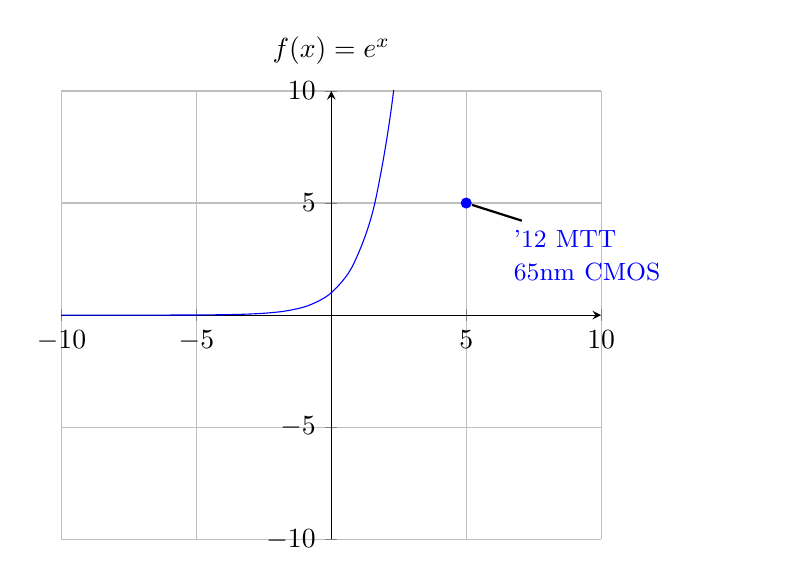
\begin{tikzpicture}
			\begin{axis} [
				axis lines = center,
				xmax = 10,
				xmin = -10,
				ymax = 10,
				ymin = -10,
				grid = major,
				title = {$f(x) = e^x$},
				restrict y to domain = -10:100
			]
				\addplot[smooth, no marks, blue, domain = -10:10] {exp(x)};
			\end{axis}
		\end{tikzpicture}
	
		\subsection*{\underline{Properties}}
		\begin{tabular}{|c|c|}
			\hline
				Domain & $(-\infty, \infty)$\\
				Range & $(0, \infty)$\\
			\hline
				Continuous & Yes\\
			\hline
				Symmetry & None\\
			\hline
				Increasing & $(-\infty, \infty)$\\
			\hline
				Bounded & Below\\
			\hline
				Extrema & None\\
			\hline
				Asymptotes & $y = 0$\\
			\hline
				Limits & \specialcell{$\lim_{x \to -\infty} f(x) = 0$\\
									  $\lim_{x \to \infty} f(x) = \infty$}\\
			\hline
		\end{tabular}
	\end{center}
	
	\subsection{Logarithmic Function}
	\begin{center}
		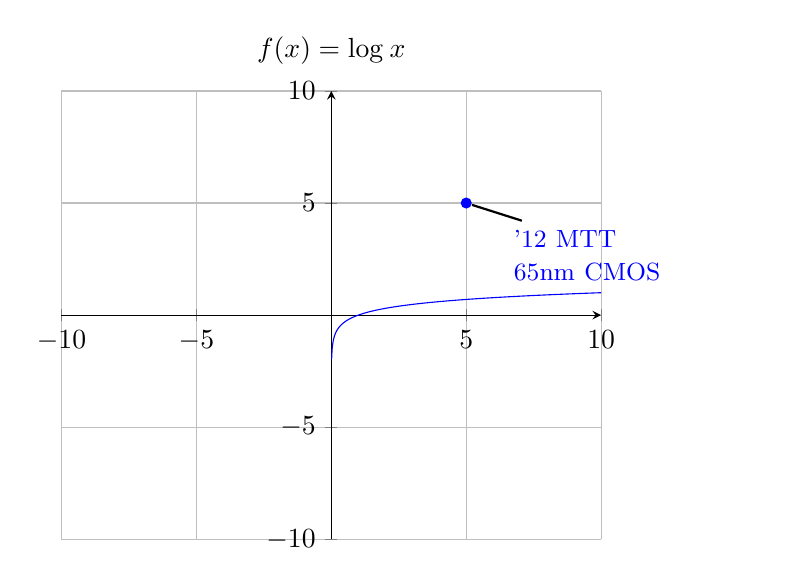
\begin{tikzpicture}
			\begin{axis} [
				axis lines = center,
				xmax = 10,
				xmin = -10,
				ymax = 10,
				ymin = -10,
				grid = major,
				title = {$f(x) = \log_{}x$},
				restrict y to domain = -10:100,
				samples = 1000
			]
				\addplot[smooth, no marks, blue, domain = -10:10] {log10(x)};
			\end{axis}
		\end{tikzpicture}
	
		\subsection*{\underline{Properties}}
		\begin{tabular}{|c|c|}
			\hline
				Domain & $(0, \infty)$\\
				Range & $(-\infty, \infty)$\\
			\hline
				Continuous & Yes\\
			\hline
				Symmetry & None\\
			\hline
				Increasing & $(0, \infty)$\\
			\hline
				Bounded & No\\
			\hline
				Extrema & None\\
			\hline
				Asymptotes & $x = 0$\\
			\hline
				Limits & \specialcell{$\lim_{x \to -\infty} f(x) = -\infty$\\
									  $\lim_{x \to \infty} f(x) = \infty$}\\
			\hline
		\end{tabular}
	\end{center}
	
	\subsection{Sine Function}
	\begin{center}
		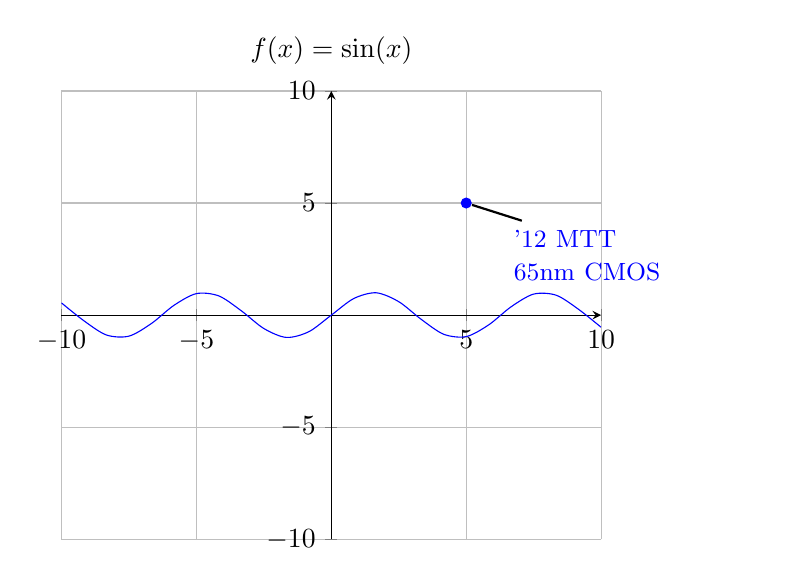
\begin{tikzpicture}
			\begin{axis} [
				axis lines = center,
				xmax = 10,
				xmin = -10,
				ymax = 10,
				ymin = -10,
				grid = major,
				title = {$f(x) = \sin(x)$},
				restrict y to domain = -10:10
			]
				\addplot[smooth, no marks, blue, domain = -10:10] {sin(deg(x))};
			\end{axis}
		\end{tikzpicture}
	
		\subsection*{\underline{Properties}}
		\begin{tabular}{|c|c|}
			\hline
				Domain & $(-\infty, \infty)$\\
				Range & $[-1, 1]$\\
			\hline
				Continuous & Yes\\
			\hline
				Symmetry & Odd\\
			\hline
				Increasing & $[-\frac{\pi}{2}, \frac{\pi}{2}]$\\
				Decreasing & $[\frac{\pi}{2}, \frac{3\pi}{2}]$\\
			\hline
				Bounded & Above and Below\\
			\hline
				Extrema & \specialcell{Minimum: $-1$\\
									   Maximum: $1$}\\
			\hline
				Asymptotes & None\\
			\hline
				Limits & \specialcell{$\lim_{x \to -\infty} f(x) = DNE$\\
									  $\lim_{x \to \infty} f(x) = DNE$}\\
			\hline
		\end{tabular}
	\end{center}
	
	\subsection{Cosine Function}
	\begin{center}
		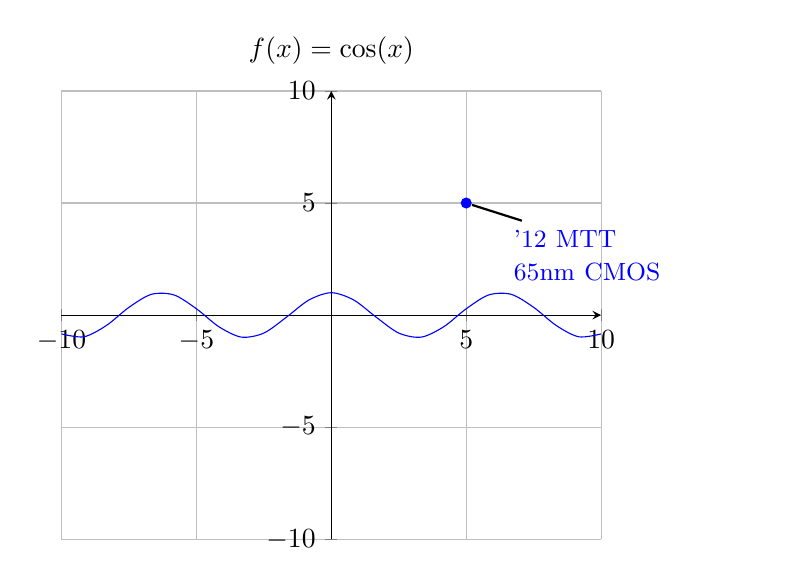
\begin{tikzpicture}
			\begin{axis} [
				axis lines = center,
				xmax = 10,
				xmin = -10,
				ymax = 10,
				ymin = -10,
				grid = major,
				title = {$f(x) = \cos(x)$},
				restrict y to domain = -10:100
			]
				\addplot[smooth, no marks, blue, domain = -10:10] {cos(deg(x))};
			\end{axis}
		\end{tikzpicture}
	
		\subsection*{\underline{Properties}}
		\begin{tabular}{|c|c|}
			\hline
				Domain & $(-\infty, \infty)$\\
				Range & $[-1, 1)$\\
			\hline
				Continuous & Yes\\
			\hline
				Symmetry & Even\\
			\hline
				Increasing & $[-\pi, 0]$\\
				Decreasing & $[0, \pi]$\\
			\hline
				Bounded & Above and Below\\
			\hline
				Extrema & \specialcell{Minimum: $-1$\\
									   Maximum: $1$}\\
			\hline
				Asymptotes & None\\
			\hline
				Limits & \specialcell{$\lim_{x \to -\infty} f(x) = DNE$\\
									  $\lim_{x \to \infty} f(x) = DNE$}\\
			\hline
		\end{tabular}
	\end{center}
	
	\subsection{Absolute Value Function}
	\begin{center}
		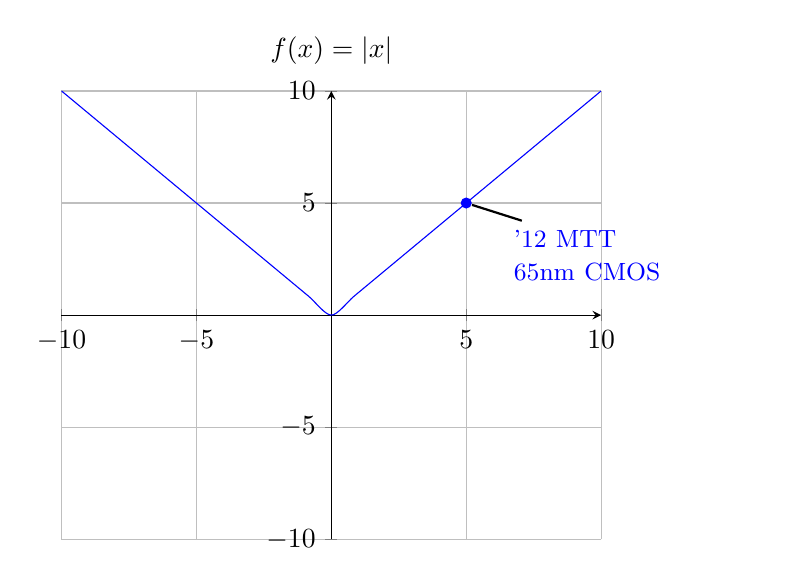
\begin{tikzpicture}
			\begin{axis} [
				axis lines = center,
				xmax = 10,
				xmin = -10,
				ymax = 10,
				ymin = -10,
				grid = major,
				title = {$f(x) = |x|$},
				restrict y to domain = -10:100
			]
				\addplot[smooth, no marks, blue, domain = -10:10] {abs(x)};
			\end{axis}
		\end{tikzpicture}
	
		\subsection*{\underline{Properties}}
		\begin{tabular}{|c|c|}
			\hline
				Domain & $(-\infty, \infty)$\\
				Range & $[0, \infty)$\\
			\hline
				Continuous & Yes\\
			\hline
				Symmetry & Even\\
			\hline
				Increasing & $[0, \infty)$\\
				Decreasing & $(-\infty, 0]$\\
			\hline
				Bounded & Below\\
			\hline
				Extrema & Minimum: $(0, 0)$\\
			\hline
				Asymptotes & None\\
			\hline
				Limits & \specialcell{$\lim_{x \to -\infty} f(x) = \infty$\\
									  $\lim_{x \to \infty} f(x) = \infty$}\\
			\hline
		\end{tabular}
	\end{center}
	
	% Because PGFPlots can do 3D graphs, but not Greatest Integer Functions
	\tikzset{
    	declare function={Floor(\x)=round(\x-0.5);}
	}
	% Styles
	\makeatletter
	\long\def\ifnodedefined#1#2#3{%
		\@ifundefined{pgf@sh@ns@#1}{#3}{#2}%
	}
	\newif\iffirstmarker
	\firstmarkertrue

	\pgfplotsset{
		discontinuous/.style={
		scatter,
		options/.style={},
		execute at end plot visualization={\global\firstmarkertrue},
		scatter/@pre marker code/.code={
		        \iffirstmarker
		            \global\firstmarkerfalse
		        \else
		    \ifnodedefined{marker}{
		        \pgfpointdiff{\pgfpointanchor{marker}{center}}%
		         {\pgfpoint{0}{0}}%
		         \ifdim\pgf@y>0pt
		            \tikzset{options/.style={mark=*}}
		            \draw plot [mark=*,mark options={fill=white}] coordinates {(marker-|0,0)};
		         \else
		            \ifdim\pgf@y<0pt
		                \tikzset{options/.style={mark=*,fill=white}}
		                \draw plot [mark=*] coordinates {(marker-|0,0)};
		            \else
		                \tikzset{options/.style={mark=none}}
		            \fi
		         \fi
		    }{
		        \tikzset{options/.style={mark=none}}        
		    }
		    \fi
		    \coordinate (marker) at (0,0);
		    \begin{scope}[options]
		},
		scatter/@post marker code/.code={\end{scope}}
		}
	}
	\subsection{Greatest Integer Function}
	\begin{center}
		\begin{tikzpicture}
			\begin{axis} [
				axis lines = center,
				xmax = 10,
				xmin = -10,
				ymax = 10,
				ymin = -10,
				grid = major,
				title = {$f(x) = int(x)$},
				restrict y to domain = -10:100,
				samples = 100
			]
				\addplot[smooth, discontinuous, no marks, jump mark left, thick, blue, domain = -10:10] {Floor(x)};
			\end{axis}
		\end{tikzpicture}
	
		\subsection*{\underline{Properties}}
		\begin{tabular}{|c|c|}
			\hline
				Domain & $(-\infty, \infty)$\\
				Range & $(0, \infty)$\\
			\hline
				Continuous & Yes\\
			\hline
				Symmetry & None\\
			\hline
				Increasing & $(-\infty, \infty)$\\
			\hline
				Bounded & Below\\
			\hline
				Extrema & None\\
			\hline
				Asymptotes & $y = 0$\\
			\hline
				Limits & \specialcell{$\lim_{x \to -\infty} f(x) = 0$\\
									  $\lim_{x \to \infty} f(x) = \infty$}\\
			\hline
		\end{tabular}
	\end{center}
	
	\subsection{Logistic Function}
	\begin{center}
		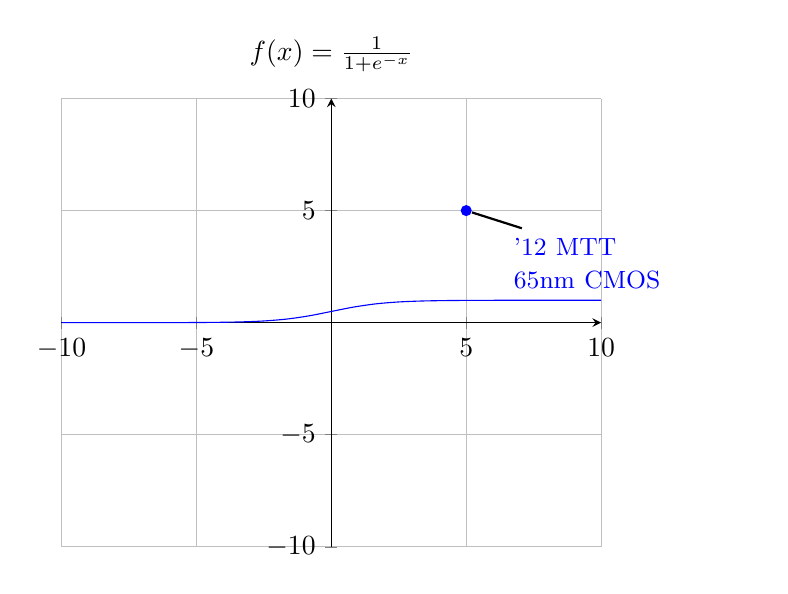
\begin{tikzpicture}
			\begin{axis} [
				axis lines = center,
				xmax = 10,
				xmin = -10,
				ymax = 10,
				ymin = -10,
				grid = major,
				title = {$f(x) = \frac{1}{1+e^{-x}}$}
			]
				\addplot[smooth, no marks, blue, domain = -10:10] {1/(1+exp(-x))};
			\end{axis}
		\end{tikzpicture}
	
		\subsection*{\underline{Properties}}
		\begin{tabular}{|c|c|}
			\hline
				Domain & $(-\infty, \infty)$\\
				Range & $(0, 1)$\\
			\hline
				Continuous & Yes\\
			\hline
				Symmetry & None\\
			\hline
				Increasing & $(-\infty, \infty)$\\
			\hline
				Bounded & Above and Below\\
			\hline
				Extrema & None\\
			\hline
				Asymptotes & \specialcell{$y = 0$\\
										  $y = 1$}\\
			\hline
				Limits & \specialcell{$\lim_{x \to -\infty} f(x) = 0$\\
									  $\lim_{x \to \infty} f(x) = 1$}\\
			\hline
		\end{tabular}
	\end{center}
	
	\pagebreak
	
	\section{Graphical Transformations}
	\subsection{Flipping the y-values over the x-axis and the y-axis}
	\begin{center}
		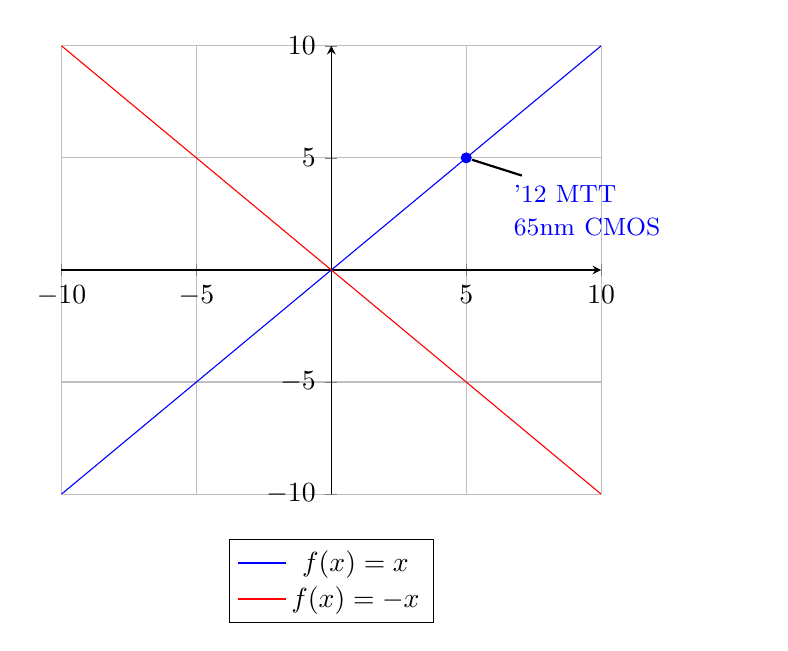
\begin{tikzpicture}
			\begin{axis} [
				axis lines = center,
				xmax = 10,
				xmin = -10,
				ymax = 10,
				ymin = -10,
				grid = major,
				legend style={at={(0.5,-0.1)},anchor=north}
			]
				\addplot[smooth, no marks, blue, domain = -10:10] {x};
				\addlegendentry{$f(x) = x$}
				\addplot[smooth, no marks, red, domain = -10:10] {-x};
				\addlegendentry{$f(x) = -x$}
			\end{axis}
		\end{tikzpicture}
	\end{center}
	
	\subsection{Moving y-values left and right on the x-axis}
	\begin{center}
		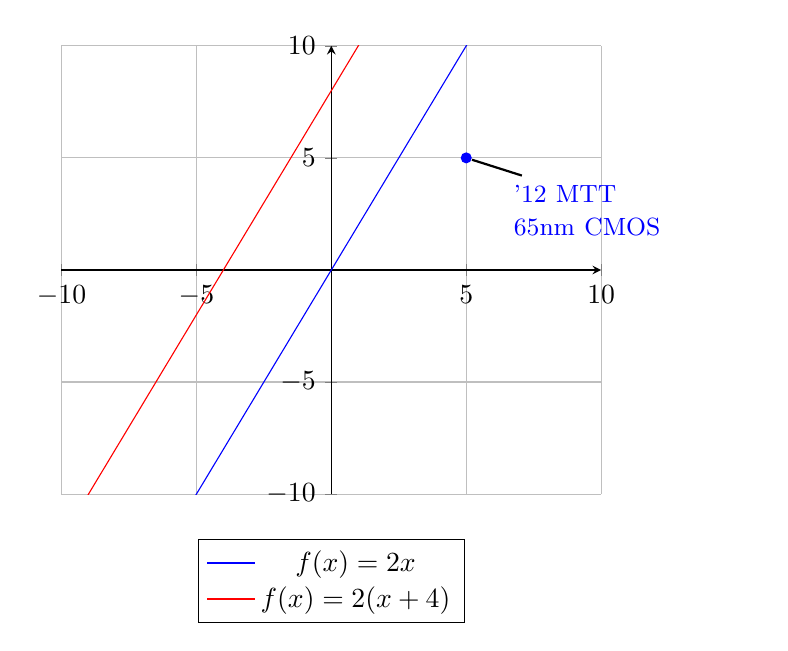
\begin{tikzpicture}
			\begin{axis} [
				axis lines = center,
				xmax = 10,
				xmin = -10,
				ymax = 10,
				ymin = -10,
				grid = major,
				legend style={at={(0.5,-0.1)},anchor=north}
			]
				\addplot[smooth, no marks, blue, domain = -10:10] {2*x};
				\addlegendentry{$f(x) = 2x$}
				\addplot[smooth, no marks, red, domain = -10:10] {2*(x+4)};
				\addlegendentry{$f(x) = 2(x+4)$}
			\end{axis}
		\end{tikzpicture}
	\end{center}
	
	\subsection{Moving the y-values up and down on the y-axis}
	\begin{center}
		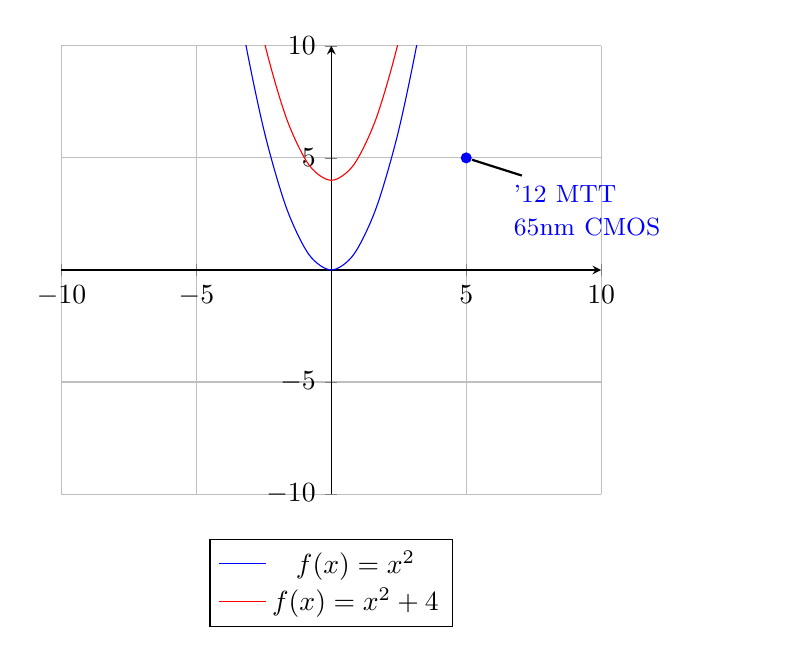
\begin{tikzpicture}
			\begin{axis} [
				axis lines = center,
				xmax = 10,
				xmin = -10,
				ymax = 10,
				ymin = -10,
				grid = major,
				legend style={at={(0.5,-0.1)},anchor=north}
			]
				\addplot[smooth, no marks, blue, domain = -10:10] {x^2};
				\addlegendentry{$f(x) = x^2$}
				\addplot[smooth, no marks, red, domain = -10:10] {x^2+4};
				\addlegendentry{$f(x) = x^2+4$}
			\end{axis}
		\end{tikzpicture}
	\end{center}
	
	\subsection{Vertical modifications to the graph}
	\subsubsection{Stretch $f(x) \rightarrow af(x)$ when $a > 1$}
	\begin{center}
		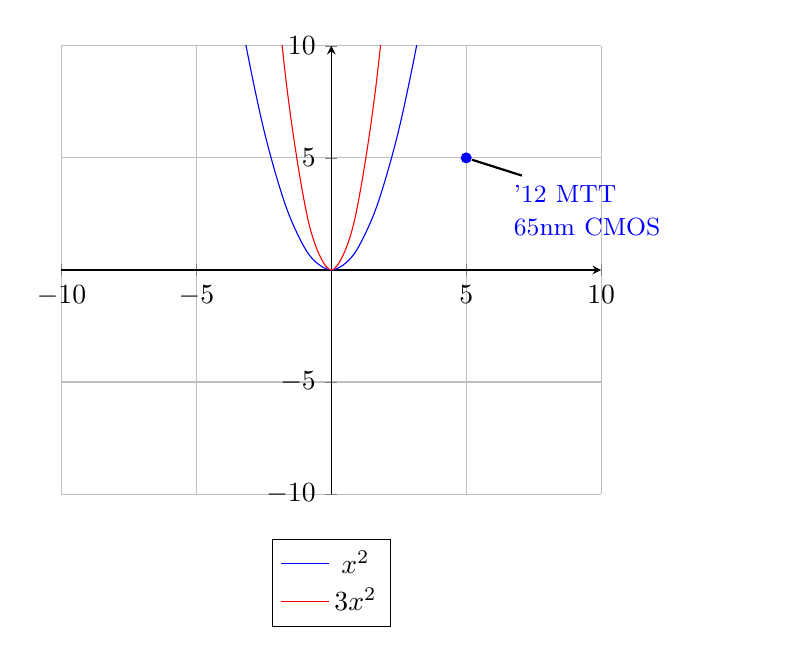
\begin{tikzpicture}
			\begin{axis} [
				axis lines = center,
				xmax = 10,
				xmin = -10,
				ymax = 10,
				ymin = -10,
				grid = major,
				legend style={at={(0.5,-0.1)},anchor=north}
			]
				\addplot[smooth, no marks, blue, domain = -10:10] {x^2};
				\addlegendentry{$x^2$}
				\addplot[smooth, no marks, red, domain = -10:10] {3*x^2};
				\addlegendentry{$3x^2$}
			\end{axis}
		\end{tikzpicture}
	\end{center}
	\subsubsection{Shrink $f(x) \rightarrow af(x)$ when $0 < a < 1$}
	\begin{center}
		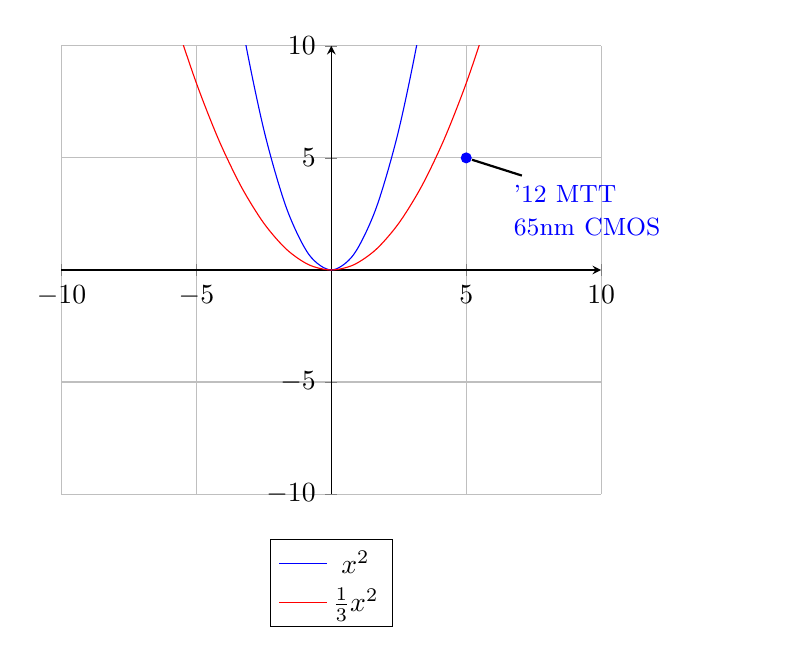
\begin{tikzpicture}
			\begin{axis} [
				axis lines = center,
				xmax = 10,
				xmin = -10,
				ymax = 10,
				ymin = -10,
				grid = major,
				legend style={at={(0.5,-0.1)},anchor=north}
			]
				\addplot[smooth, no marks, blue, domain = -10:10] {x^2};
				\addlegendentry{$x^2$}
				\addplot[smooth, no marks, red, domain = -10:10] {1/3*x^2};
				\addlegendentry{$\frac{1}{3}x^2$}
			\end{axis}
		\end{tikzpicture}
	\end{center}
	\subsection{Horizontal modifications to the graph}
	\subsubsection{Stretch $f(x) \rightarrow f(x\div c)$ when $c > 1$}
	\begin{center}
		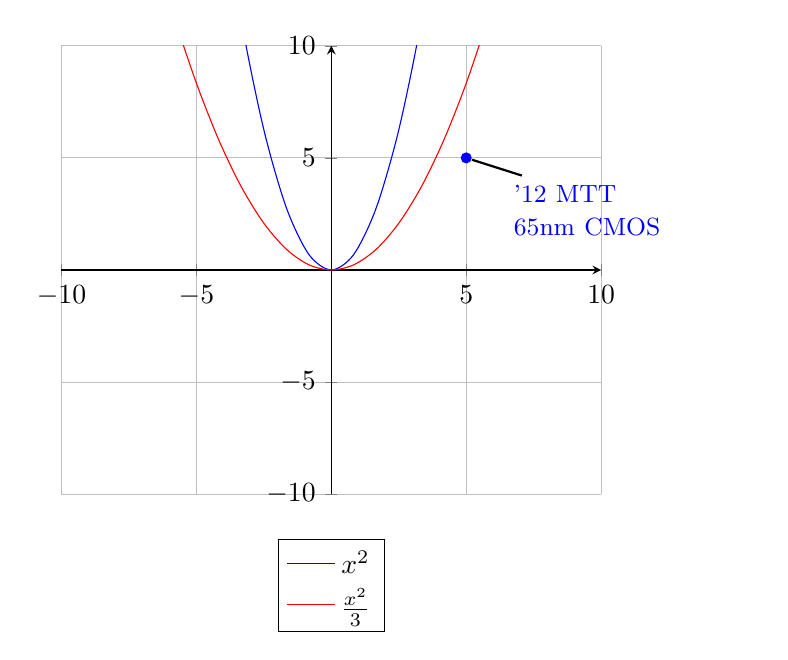
\begin{tikzpicture}
			\begin{axis} [
				axis lines = center,
				xmax = 10,
				xmin = -10,
				ymax = 10,
				ymin = -10,
				grid = major,
				legend style={at={(0.5,-0.1)},anchor=north}
			]
				\addplot[smooth, no marks, blue, domain = -10:10] {x^2};
				\addlegendentry{$x^2$}
				\addplot[smooth, no marks, red, domain = -10:10] {(x^2)/3};
				\addlegendentry{$\frac{x^2}{3}$}
			\end{axis}
		\end{tikzpicture}
	\end{center}
	\subsubsection{Shrink $f(x) \rightarrow f(x\div c)$ when $0 < c < 1$}
	\begin{center}
		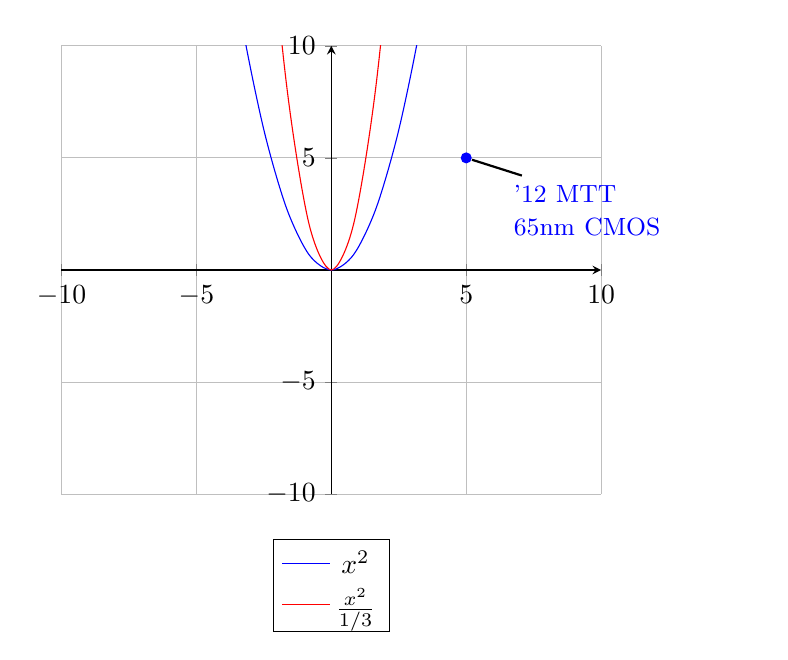
\begin{tikzpicture}
			\begin{axis} [
				axis lines = center,
				xmax = 10,
				xmin = -10,
				ymax = 10,
				ymin = -10,
				grid = major,
				legend style={at={(0.5,-0.1)},anchor=north}
			]
				\addplot[smooth, no marks, blue, domain = -10:10] {x^2};
				\addlegendentry{$x^2$}
				\addplot[smooth, no marks, red, domain = -10:10] {(x^2)/(1/3)};
				\addlegendentry{$\frac{x^2}{1/3}$}
			\end{axis}
		\end{tikzpicture}
	\end{center}
	\section{Function Composition and Inverse}
	\subsection{Function Composition}
	Composing functions is as simple as substituting the selected function's $x$ value with the other equation.
	\subsubsection*{Example: $f(x) = 2x^2-x$ and $g(x) = x^3$}
	\begin{center}
		\begin{tabular}{|c|c|c|}
			\hline
				Old Functions and Domains & $f(x) = 2x^2-x$ & $(-\infty, \infty)$ \\
				& $g(x) = x^3$ & $(-\infty, \infty)$ \\
			\hline
				New Functions and Domains & $(fog)(x) = 2x^{6}-x^3$ & $(-\infty, \infty)$ \\
				& $(gof)(x) = (2x^2-x)^3$ & $(-\infty, \infty)$ \\
			\hline
		\end{tabular}
	\end{center}
	\subsubsection*{Example: $f(x) = 3x+1$ and $g(x) = \frac{1}{x}$}
	\begin{center}
		\begin{tabular}{|c|c|c|}
			\hline
				Old Functions and Domains & $f(x) = 3x+1$ & $(-\infty, \infty)$ \\
				& $g(x) = \frac{1}{x}$ & $(-\infty, 0)\bigcup(0, \infty)$ \\
			\hline
				New Functions and Domains & $(fog)(x) = 3(\frac{1}{3}+1)$ & $(-\infty, \infty)$ \\
				& $(gof)(x) = \frac{1}{3x+1}$ & $(-\infty, \infty)$ \\
			\hline
		\end{tabular}
	\end{center}
	\subsection{Inverse}
	\subsubsection*{Example: $y = 9x+2$}
	To get the inverse of a function, simply replace the $x$ and the $y$ in the equation to get your inverse. The end result should be simplified
	to get $y$ back on the other side.
	\begin{center}
		\begin{tabular}{|c|c|c|}
			\hline
				Old Function and Domain & $y = 9x+2$ & $(-\infty, \infty)$ \\
			\hline
				New Function and Domain & $y^{-1} = \frac{x-2}{9}$ & $(-\infty, \infty)$ \\
			\hline
		\end{tabular}
	\end{center}
	\subsubsection*{Example: $y = \sqrt{x^3+4}$}
	\begin{center}
		\begin{tabular}{|c|c|c|}
			\hline
				Old Function and Domain & $y = \sqrt{x^3+4}$ & $\left[\sqrt[3]{-4}, \infty\right)$ \\
			\hline
				New Function and Domain & $y^{-1} = \sqrt[3]{x^2-4}$ & $(-\infty, \infty)$ \\
			\hline
		\end{tabular}
	\end{center}
	\section{Quadratic Functions}
	\subsection{Standard Form}
	Standard form is beneficial for seeing transformations, and other manipulations of the graph. It's also a form that's easily factorable if needed.
	\subsubsection*{$f(x) = ax^2+bx+c$}
	\subsection{Vertex Form}
	Vertex form is good for finding the vertex and axis of symmetry with ease. It's much harder to factor, but can be transformed
	into \underline{Standard Form} if needed be. \textbf{Vertex: $(h, k)$}
	\subsubsection*{$f(x) = a(x-h)^2+k$}
	\subsection{Converting from Standard Form to Vertex Form using Completing the Square}
	\begin{center}
		\begin{tabular}{|c|c|}
			\hline
				Starting equation & $y = 2x^2-4x+5$ \\
			\hline
				\specialcell{To complete the square,\\
				our $x^2$ and $x$ terms\\
				must be isolated.} & $y - 5 = 2x^2 - 4x$ \\
			\hline
				\specialcell{The leading coefficient\\
				must be $1$ to continue. Let's\\
				factor out the leading\\
				coefficient of 2.} & $y - 5 = 2(x^2-2x)$ \\
			\hline
				\specialcell{We need a perfect square\\
				trinomial.} & $y - 5 + 2 \fbox{\phantom{x}} = 2\left(x^2-2x+\fbox{\phantom{x}} \right)$ \\
			\hline
				\specialcell{Find the perfect trinomial\\
				by taking half of the coefficient \\
				of the $x$ term, squaring it, \\
				and putting it in the boxes.} & $y - 5 + 2 \fbox{1} = 2\left(x^2-2x+\fbox{1} \right)$ \\
			\hline
				\specialcell{Simplify and make the right\\
				side a square expression.} & $y - 3 = 2(x-1)^2$ \\
			\hline
				\specialcell{Isolate the $y$ term by\\
				moving the $-3$ to the other side.} & $y = 2(x-1)^2 + 3$ \\
			\hline
		\end{tabular}
	\end{center}
	\section{Power Functions}
	A power function must have a degree greater than 2, it must be a monomial, and the exponents can be positive or negative.
	\subsection{Direct Variation}
	Direct variation is good for modeling equations where when one variable increases or decreases, the resulting value will do the same
	based on a predetermined ratio.
	\subsubsection*{A couch factory makes 12 couches per hour. If the amount of hours
	given increases, so will the total amount of couches made.}
	A direct variation can only exist if the degree is positive.
	\subsubsection*{Example: $c = 12h$}
	This example models the real world example about the couch factory. The $12$ is the constant of variation, and the exponent of our $h$
	term (1) is the degree.
	\subsection{Indirect Variation}
	Indirect variation is good for modeling equations where when one variable increases or decreases, the resulting value will do the opposite
	based on a predetermined ration.
	\subsubsection*{As the volume of a container increases, the pressure decreases.}
	An indirect variation can only exist if the degree is negative.
	\subsubsection*{Example: $k = P/V$}
	This example models the real world example about the gas's pressure. The $P$ is the pressure variable and the $V$ is the volume variable.
	The constant of variation is our numerator ($P$) and the degree is the opposite of our denominator's exponent (-1).
	\section{Polynomial Functions}
	\subsection{Multiplicity}
	Multiplicity is the number of times a function has a zero at a certain point. It helps us by giving us a rough sketch of what the graph will
	look like.
	\subsubsection{Guesstimating a graph from: $(x-1)^2(x+3)^3(x+4)$}
	The key factor in what a graph will do is based on the exponent on each term. Use the following table to determine what the graph will do:
	\begin{center}
		\begin{tabular}{|c|c|}
			\hline
				Exponent is 1 & \specialcell{The graph will go straight through\\
				at this point.} \\
			\hline
				Exponent is 2 & \specialcell{The graph will bounce off this point,\\
				similar to a parabola.} \\
			\hline
				Exponent is 3 & \specialcell{The graph will curve through this\\
				point, similar to how $y = x^3$ looks.} \\
			\hline
		\end{tabular}
	\end{center}
	If the exponent goes higher than the table explains, if the exponent is event it follows the 2nd rule, and if the exponent is odd it follows
	the third rule.
	\subsubsection*{Actual Graph}
	\begin{center}
		\begin{tikzpicture}
			\begin{axis} [
				axis lines = center,
				xmax = 1.8,
				xmin = -4.2,
				ymax = 150,
				ymin = -10,
				grid = major,
				restrict y to domain=-10:150
			]
				\addplot[smooth, no marks, blue, domain = -10:10] {((x-1)^2)*((x+3)^3)*(x+4)};
			\end{axis}
		\end{tikzpicture}
	\end{center}
	As you can see, the graph is close to our predictions, but isn't exact. Using multiplicity to guesstimate our graph is just that: Guesstimating.
	As you've also probably noticed, our $y$ values are quite large, another downfall of guesstimating of graphs is we can't get $y$ values
	without plugging in the $x$ value which takes lots of effort and time.
	\subsection{Finding the function from zeros}
	We can also look at the graph and turn it into a function by finding the zeros of the function. By following our rules we can find the equation
	of our graph real easily.
	\subsubsection*{Example Graph}
		\begin{center}
		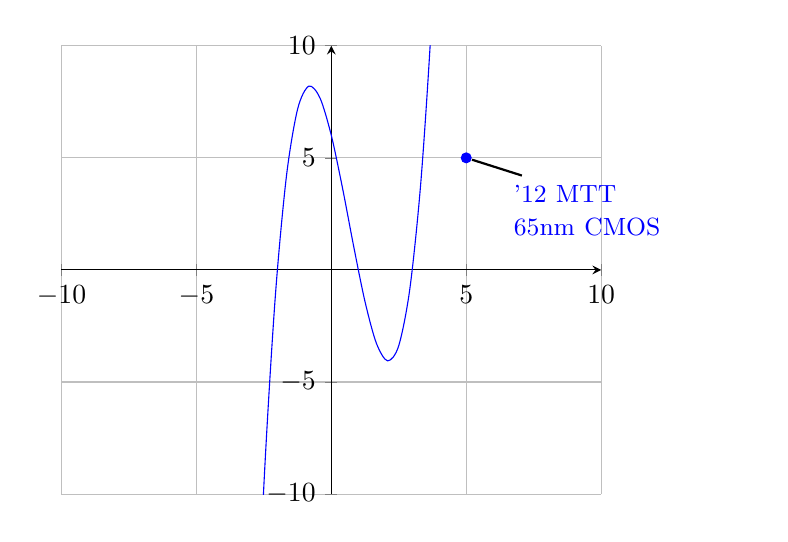
\begin{tikzpicture}
			\begin{axis} [
				axis lines = center,
				xmax = 10,
				xmin = -10,
				ymax = 10,
				ymin = -10,
				grid = major,
			]
				\addplot[smooth, no marks, blue] {(x-1)*(x-3)*(x+2)};
			\end{axis}
		\end{tikzpicture}
	\end{center}
	By finding where $x = 0$ and knowing that all three zeros go straight through the $y$ axis, we can solidify this information into an equation
	that looks something like $(x-3)(x-1)(x+2)$.
	\section{Long Division vs. Synthetic Division}
	Long division can be helpful for when synthetic division may not work, but other than that, it's very verbose and isn't the preferred method of
	polynomial division. Synthetic division is much more helpful (when it works) because you can get a remainder as well as an answer very
	quickly by simply multiplying the previous term with the current term, getting the sum, and repeating until you get to the end.
	\subsection{Long Divison Example}
	\polylongdiv{x^2-9x-10}{x+1}
	\subsection{Synthetic Division Example}
	\polyhornerscheme[x=-1]{x^2-9x-10}\\
	The last column is our remainder, and the first two can transform into our final answer: $x - 10$.
	\section{Solving Inequalities With Sign Charts}
	\subsection*{Example: $\frac{(x-5)(x+1)^2}{(x+3)(x-3)}$}\vspace{5mm}
	\sgchart{~-3, -1, ~3, 5}{\frac{(x-5)(x+1)^2}{(x+3)(x-3)}: -++-+}\vspace{5mm}
	\begin{center}
		\begin{tabular}{|c|c|}
			\hline
				$f(x) > 0$ & $(-3, -1)\bigcup(-1, 3)\bigcup(5, \infty)$ \\
			\hline
				$f(x) \geq 0$ & $(-3, 3)\bigcup[5, \infty)$ \\
			\hline
				$f(x) < 0$ & $(-\infty, -3)\bigcup(3, 5)$ \\
			\hline
				$f(x) \leq 0$ & $(-\infty, -3)\bigcup[-1]\bigcup(3, 5]$ \\
			\hline
		\end{tabular}
	\end{center}\vspace{5mm}
	By using this sign chart, we've come up with inequalities for the function.
	\section{Exponential and Logarithmic Functions}
	\subsection{Solving Exponential Functions}
	Exponential and Logarithmic functions are great for when the rate of change needs to change dynamically.
	\begin{center}
		Exponential: $y = ab^x$\\
		$a$ = initial value\\
		$b$ = growth or decay factor\\
		Growth if $b > 1$\\
		Decay if $0 < b < 1$
	\end{center}
	\subsubsection*{Example: Chicago has a population of 1.5 million in 2007. The population grows 2.6\% every year.}
	The equation is structured as follows:
	\begin{center}
		$current point = starting point * (growth / decay factor)^{years since starting year}$
	\end{center}
	Which means our equation would look something like:
	\begin{center}
		$y = 1500000*1.026^x$
	\end{center}
	\subsection{Solving Logarithmic Functions}
	Logarithmic functions can be solved by hand in certain cases, but most logistic functions will need to be solved by the calculator.
	All logarithmic functions can be solved very easily with your calculator by typing $log(your number)$. But to do it by hand, you must
	find an equation that'll cancel.
	\begin{center}
		\sout{$log_{10}10^2$} $= 2$
	\end{center}
	As you can see, the tens cancel out and leaves you with a $2$. As this isn't usually the case, keep a calculator nearby!
	\subsection{Properties of Logs}
	\subsubsection{Condensing}
	\begin{center}
		$4log(xy)-3log(yz) \to \frac{4logxy}{3logyz} \to \frac{log(xy)^4}{log(yz)^3} \to log\frac{x^4y^4}{z^3y^3} \to log\frac{x^4y}{z^3}$
	\end{center}
	\subsubsection{Expanding}
	\begin{center}
		$log\frac{x^4y}{z^3} \to log\frac{x^4y^4}{z^3y^3} \to \frac{log(xy)^4}{log(yz)^3} \to \frac{4logxy}{3logyz} \to 4log(xy)-3log(yz)$
	\end{center}
	\section{Partial Fraction Decomposition}
	\begin{enumerate}
		\item Factor the denominator
		\item If you have a linear factor:\vspace{5mm}
		\textbf{Decompose:}\\
		$\frac{A_1}{mx+b} + \frac{A_2}{(mx+b)^2} + \dots$
		\item If you have a quadratic factor:\vspace{5mm}
		\textbf{Decompose:}\\
		$\frac{B_1X+C}{ax^2+bx+c}+\frac{B_2X+C_2}{(ax^2+bx+c)^2}+\dots$
		\item Get a common denominator and solve for your variables
	\end{enumerate}
	\subsection{Decompose: $\frac{5x-1}{x^2-2x-15} = \frac{5x-1}{(x-5)(x+3)}$}
	$\frac{A_1}{x-5} + \frac{A_2}{x+3} = \frac{5x-1}{(x-4)(x+3)}$\\ \vspace{5mm}
	$A_1(x+3) + A_2(x-5) = 5x - 1$\\ \vspace{5mm}
	$\textcolor{blue}{A_1x} + \textcolor{red}{3A_1}+\textcolor{blue}{A_2x}\textcolor{red}{-5A_2}=\textcolor{blue}{5x}\textcolor{red}{-1}$\\
	\vspace{5mm}
	$A_1+A_2=5$\\ \vspace{5mm}
	$3A_1-5A_2=-1$\\ \vspace{5mm}
	$3(3)-5(2)=-1$\\ \vspace{5mm}
	$9 - 10=-1$\\
	\begin{center}
	\fbox{\begin{varwidth}{\textwidth}
		$A_1 = 3 \\
		A_2 = 2$
	\end{varwidth}
	}
	$\to$
	\fbox{\begin{varwidth}{\textwidth}
		$\frac{3}{x-5} + \frac{2}{x+3}$
	\end{varwidth}
	}
	\end{center}
	\subsection{Sequences and Series}
	\subsubsection{Sequences}
	\begin{center}
		\begin{tabular}{|c|c|c|}
			\hline
				& \textbf{Arithmetic Sequences} & \textbf{Geometric Sequences} \\
			\hline
				Recursive Formula & $a_n=a_{n-1}+d$ & $a_n=a_{n-1}*r$ \\
			\hline
				Explicit Formula & $a_n=a_1+d(n-1)$ & $a_n=a_1*r^{n-1}$ \\
			\hline
		\end{tabular}
	\end{center}
	\subsection{Convergent vs. Divergent Sequences}
	A convergent series will be limited by a number. For example:
	\begin{center}
		$1$\foreach \i in {2, 3, ..., 5} {$\frac{1}{\i}$}
	\end{center}
	is limited to 0.\\
	While something like:
	\begin{center}
		\foreach \i in {5, 7, ..., 13} {$\i,$} $\dots , 2n + 3$
	\end{center}
	isn't limited (or has a limit of $\infty$) allowing it to continue forever.
	\subsection{Sum of Finite Series}
	\subsubsection*{Example: $29 + 24 + 19 + 14$}
	\begin{center}
		$\mathlarger{\mathlarger{\sum}}_{k=1}^{4} -5k+34 = 89$
	\end{center}
	\subsubsection*{Example: $1 + 8 + 27 + 64 + 125$}
	\begin{center}
		$\mathlarger{\mathlarger{\sum}}_{k=1}^{5} k^3 = 225$
	\end{center}
	\subsection{Partial Sum of Infinite Series}
	\subsubsection*{Example: $S_\infty = \frac{9}{1-r}$}
	\begin{center}
		$\mathlarger{\mathlarger{\sum}}_{k=1}^{\infty} 3(\frac{3}{10})^{k-1}$
	\end{center}
	\section{Trigonometric Functions}
	\subsection{Radians}
	\subsubsection*{Radians to Degrees: $\frac{3\pi}{2}$}
	\begin{center}
		$\frac{3\pi}{2} * \frac{180}{\pi} = 270\degree$
	\end{center}
	To convert radians to degrees, you multiply it by $\frac{180}{\pi}$.
	\subsubsection*{Degrees to Radians: $360\degree$}
	\begin{center}
		$360 * \frac{\pi}{180} = 2\pi$
	\end{center}
	\subsection{Unit Circle}
	The unit circle is a model which helps with calculating values of trigonometric functions by hand.
	\begin{center}
	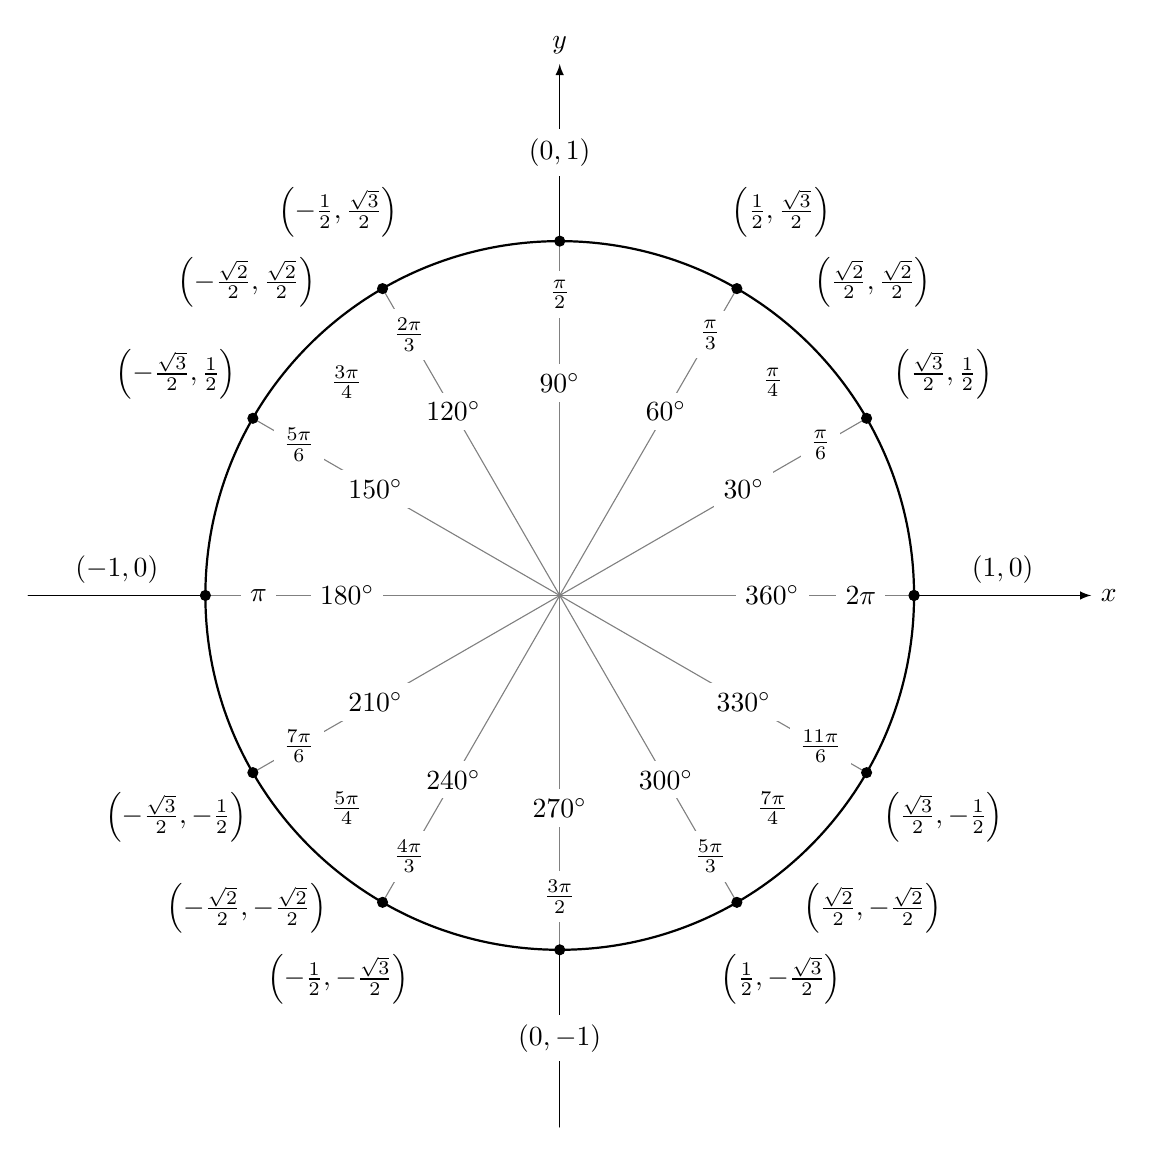
\begin{tikzpicture}[scale=4.5,cap=round,>=latex]
	% draw the coordinates
	\draw[->] (-1.5cm,0cm) -- (1.5cm,0cm) node[right,fill=white] {$x$};
	\draw[->] (0cm,-1.5cm) -- (0cm,1.5cm) node[above,fill=white] {$y$};

	% draw the unit circle
	\draw[thick] (0cm,0cm) circle(1cm);

	\foreach \x in {0,30,...,360} {
		% lines from center to point
		\draw[gray] (0cm,0cm) -- (\x:1cm);
		% dots at each point
		\filldraw[black] (\x:1cm) circle(0.4pt);
		% draw each angle in degrees
		\draw (\x:0.6cm) node[fill=white] {$\x^\circ$};
        }

	% draw each angle in radians
	\foreach \x/\xtext in {
		30/\frac{\pi}{6},
		45/\frac{\pi}{4},
		60/\frac{\pi}{3},
		90/\frac{\pi}{2},
		120/\frac{2\pi}{3},
		135/\frac{3\pi}{4},
		150/\frac{5\pi}{6},
		180/\pi,
		210/\frac{7\pi}{6},
		225/\frac{5\pi}{4},
		240/\frac{4\pi}{3},
		270/\frac{3\pi}{2},
		300/\frac{5\pi}{3},
		315/\frac{7\pi}{4},
		330/\frac{11\pi}{6},
		360/2\pi}
		\draw (\x:0.85cm) node[fill=white] {$\xtext$};

	\foreach \x/\xtext/\y in {
		% the coordinates for the first quadrant
		30/\frac{\sqrt{3}}{2}/\frac{1}{2},
		45/\frac{\sqrt{2}}{2}/\frac{\sqrt{2}}{2},
		60/\frac{1}{2}/\frac{\sqrt{3}}{2},
		% the coordinates for the second quadrant
		150/-\frac{\sqrt{3}}{2}/\frac{1}{2},
		135/-\frac{\sqrt{2}}{2}/\frac{\sqrt{2}}{2},
		120/-\frac{1}{2}/\frac{\sqrt{3}}{2},
		% the coordinates for the third quadrant
		210/-\frac{\sqrt{3}}{2}/-\frac{1}{2},
		225/-\frac{\sqrt{2}}{2}/-\frac{\sqrt{2}}{2},
		240/-\frac{1}{2}/-\frac{\sqrt{3}}{2},
		% the coordinates for the fourth quadrant
		330/\frac{\sqrt{3}}{2}/-\frac{1}{2},
		315/\frac{\sqrt{2}}{2}/-\frac{\sqrt{2}}{2},
		300/\frac{1}{2}/-\frac{\sqrt{3}}{2}}
		\draw (\x:1.25cm) node[fill=white] {$\left(\xtext,\y\right)$};

	% draw the horizontal and vertical coordinates
	% the placement is better this way
	\draw (-1.25cm,0cm) node[above=1pt] {$(-1,0)$}
		(1.25cm,0cm)  node[above=1pt] {$(1,0)$}
		(0cm,-1.25cm) node[fill=white] {$(0,-1)$}
		(0cm,1.25cm)  node[fill=white] {$(0,1)$};
	\end{tikzpicture}
	\end{center}
	\subsection{Graphs of Cosecant, Secant, and Cotangent}
	\subsubsection{Cosecant}
	\begin{center}
	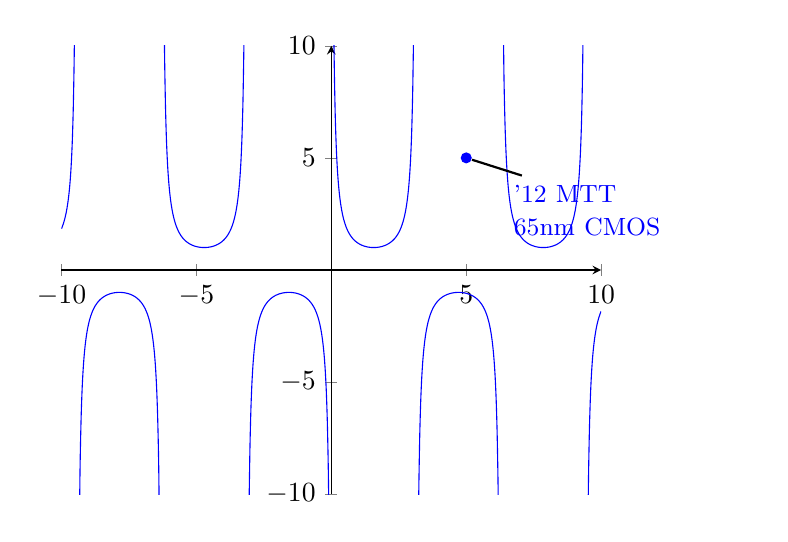
\begin{tikzpicture}
		\begin{axis}[every axis plot post/.append style={
			mark=none,
			domain=-10:10,
			samples=500,
			smooth},
		axis x line=middle,
		axis y line=center,
		xmin=-10,
		xmax=10,
		ymin=-10,
		ymax=10,
		restrict y to domain = -30:30]
			\addplot {cosec(deg(x))};
		\end{axis}
	\end{tikzpicture}
	\end{center}
	\subsubsection{Secant}
	\begin{center}
	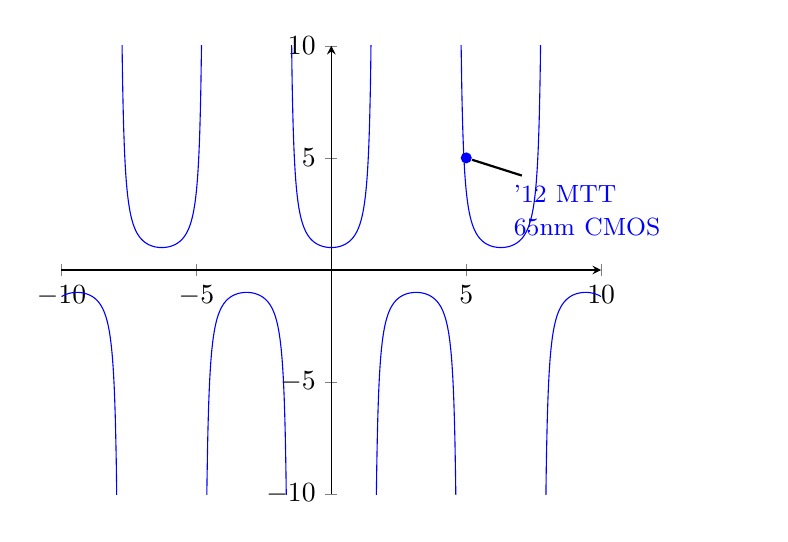
\begin{tikzpicture}
		\begin{axis}[every axis plot post/.append style={
			mark=none,
			domain=-10:10,
			samples=500,
			smooth},
		axis x line=middle,
		axis y line=center,
		xmin=-10,
		xmax=10,
		ymin=-10,
		ymax=10,
		restrict y to domain = -30:30]
			\addplot {sec(deg(x))};
		\end{axis}
	\end{tikzpicture}
	\end{center}
	\subsubsection{Cotangent}
	\begin{center}
	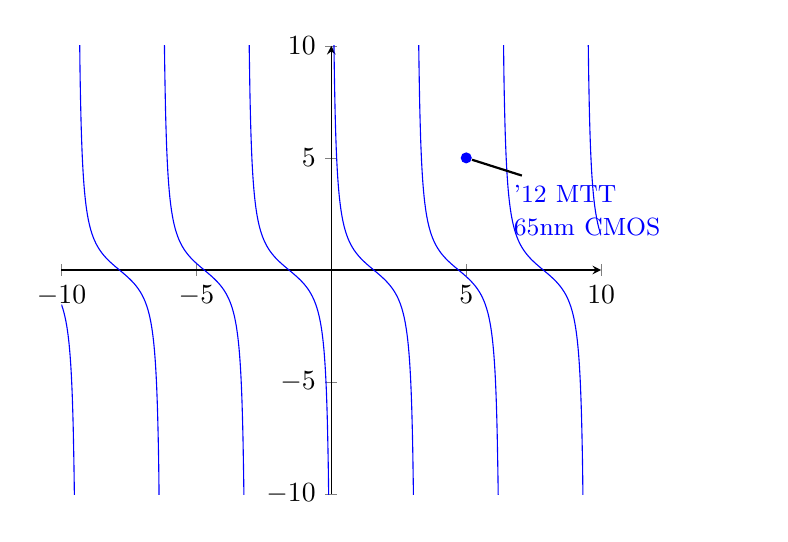
\begin{tikzpicture}
		\begin{axis}[every axis plot post/.append style={
			mark=none,
			domain=-10:10,
			samples=500,
			smooth},
		axis x line=middle,
		axis y line=center,
		xmin=-10,
		xmax=10,
		ymin=-10,
		ymax=10,
		restrict y to domain = -30:30]
			\addplot {cot(deg(x))};
		\end{axis}
	\end{tikzpicture}
	\end{center}
	\subsection{Inverse Sine, Cosine, Tangent}
	\subsubsection{Inverse Sine}
	\begin{center}
		\begin{tikzpicture}
			\begin{axis}[domain = -1:1,
				samples = 500,
				axis x line = middle,
				axis y line = middle,
				xmin = -1,
				xmax = 1,
				ymin = -180,
				ymax = 180]
				\addplot[color = red]  {asin(x)};
			\end{axis}
		\end{tikzpicture}
	\end{center}
	\subsubsection{Inverse Cosine}
	\begin{center}
		\begin{tikzpicture}
			\begin{axis}[domain = -1:1,
				samples = 500,
				axis x line = middle,
				axis y line = middle,
				xmin = -1,
				xmax = 1,
				ymin = 0,
				ymax = 180]
				\addplot[color = red]  {acos(x)};
			\end{axis}
		\end{tikzpicture}
	\end{center}
	\subsubsection{Inverse Tangent}
	\begin{center}
		\begin{tikzpicture}
			\begin{axis}[domain = -1:1,
				samples = 500,
				axis x line = middle,
				axis y line = middle,
				xmin = -1,
				xmax = 1,
				ymin = -90,
				ymax = 90]
				\addplot[color = red]  {atan(x)};
			\end{axis}
		\end{tikzpicture}
	\end{center}
	\subsection{Evaluating Trigonometry Expressions Using The Unit Circle}
	\subsubsection*{Example: $\sin{-300}$}
	If you look at the unit circle, you'll notice that $-300\degree$ isn't on it. This means we need to find a coterminal angle. To find a
	coterminal angle, we need to add (or subtract if it's higher than 360) an entire circle. Adding $360\degree$ to $-300\degree$ results
	in $60\degree$. If we look at the sine value ($y-value$) for $60\degree$ we get $\frac{\sqrt{3}}{2}$.
	\subsubsection*{Example: $\cos{-630}$}
	As this is another negative angle, we need to add $360\degree$ to the angle. After adding $360\degree$ you'll see that it's still a negative
	angle, sometimes we need to add $360\degree$ more than once. So let's add it again and get $90\degree$. Looking at the cosine
	value ($x value$) for $90\degree$ we get $0$.
	\subsubsection*{Example: $\tan(-135)$}
	Getting the coterminal angle gives us $225\degree$, and because we know $\tan(x) = \frac{sin(x)}{\cos(x)}$ we can see that
	$225\degree = 1$.
	\subsubsection*{Example: $csc(\frac{3\pi}{2})$}
	Sense $\frac{3\pi}{2}$ is on our unit circle, we don't need to find any coterminal angles. Because cosecant is $\frac{1}{sin(x)}$ we
	take the $-1$ (the $sine value of 270\degree$) and we get $\frac{1}{-1}$ which can be simplified to $-1$.
	\subsubsection*{Example: $sec(\frac{\pi}{2})$}
	$sec(\frac{\pi}{2})$ is on our unit circle, and because $sec(x) = \frac{1}{cos(x)}$ we know that $sec(\frac{\pi}{2}) = \frac{1}{0}$.
	Because anything divided by $0$ can't be done, our answer is undefined.
	\subsubsection*{Example: $cot(\pi)$}
	We know that $cot(x) = \frac{\cos(x)}{\sin{x}}$ so by using this function we can find that $cot(\pi) = \frac{-1}{0}$. And once again, because
	we know anything divided by $0$ is undefined, our answer is undefined.
	\subsubsection*{Example: $sin^{-1}(0)$}
	Any trigonometry function (except $cos(x)$, $sec(x)$, and $cos^{-1}(x)$) of $0$ regardless of degrees or radians is $0$. Because this
	is an inverse sine function, our answer is $0$.
	\subsubsection*{Example: $cos^{-1}(0.5)$}
	Our $x-value$ is $\frac{1}{2}$ at $60\degree$.
	\subsubsection*{Example: $tan^{-1}(1)$}
	Our $\frac{y-value}{x-value}$ is $1$ at $45\degree$.
	\subsection{Sinusoidal Functions}
	\subsubsection*{Amplitute}
	\begin{center}
		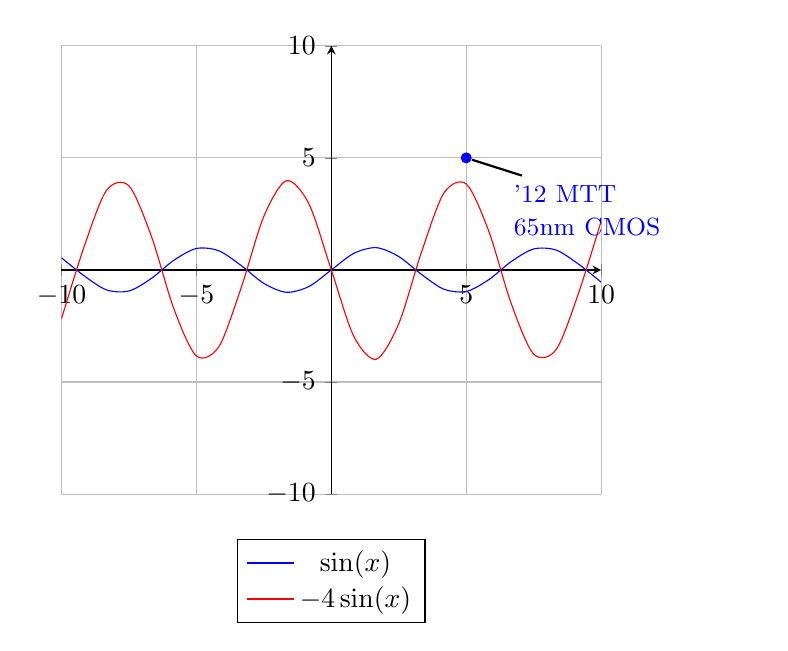
\begin{tikzpicture}
			\begin{axis} [
				axis lines = center,
				xmax = 10,
				xmin = -10,
				ymax = 10,
				ymin = -10,
				grid = major,
				legend style={at={(0.5,-0.1)},anchor=north}
			]
				\addplot[smooth, no marks, blue, domain = -10:10] {sin(deg(x))};
				\addlegendentry{$\sin(x)$}
				\addplot[smooth, no marks, red, domain = -10:10] {-4*sin(deg(x))};
				\addlegendentry{$-4\sin(x)$}
			\end{axis}
		\end{tikzpicture}
	\end{center}
	\subsubsection*{Period}
	\begin{center}
		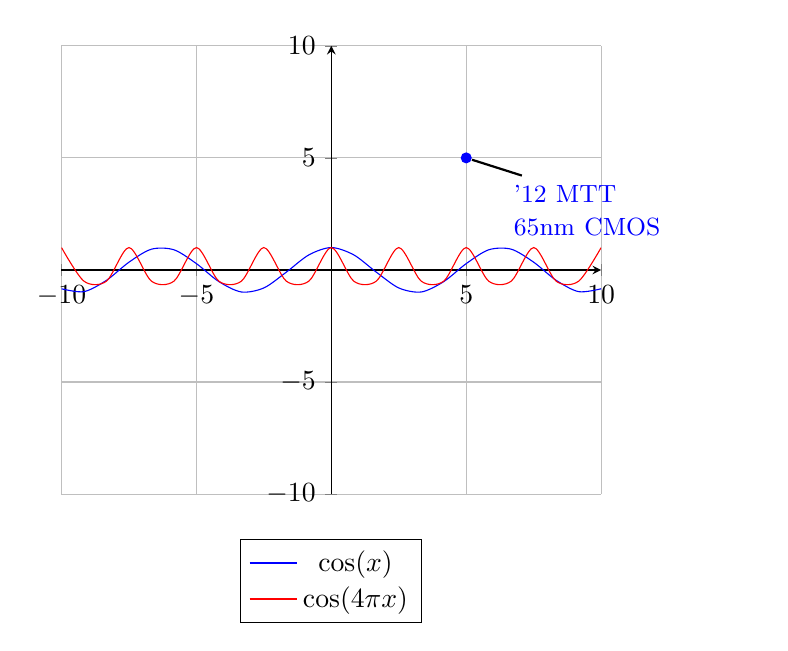
\begin{tikzpicture}
			\begin{axis} [
				axis lines = center,
				xmax = 10,
				xmin = -10,
				ymax = 10,
				ymin = -10,
				grid = major,
				legend style={at={(0.5,-0.1)},anchor=north}
			]
				\addplot[smooth, no marks, blue, domain = -10:10] {cos(deg(x))};
				\addlegendentry{$\cos(x)$}
				\addplot[smooth, no marks, red, domain = -10:10] {cos(deg(4*pi*x))};
				\addlegendentry{$\cos(4\pi x)$}
			\end{axis}
		\end{tikzpicture}
	\end{center}
	\subsubsection*{Phase Shift}
	\begin{center}
		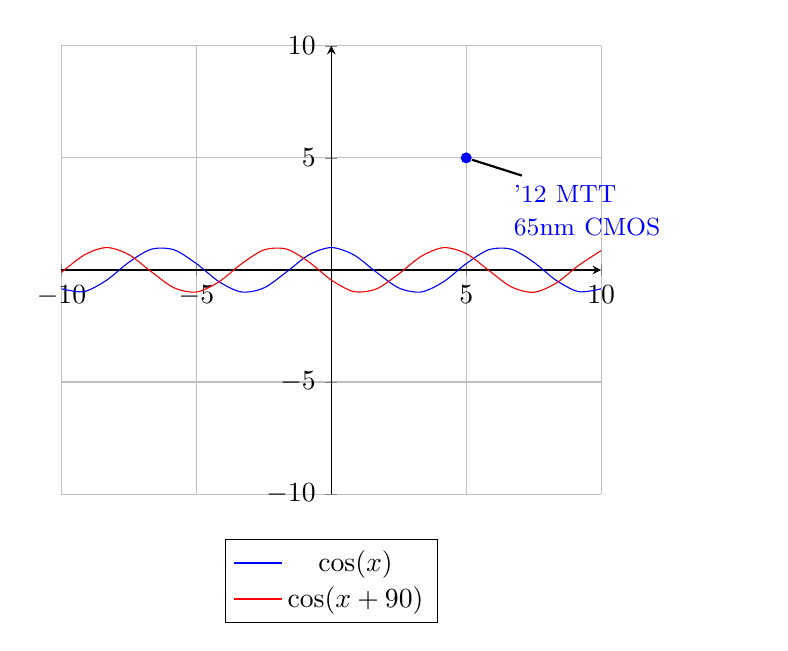
\begin{tikzpicture}
			\begin{axis} [
				axis lines = center,
				xmax = 10,
				xmin = -10,
				ymax = 10,
				ymin = -10,
				grid = major,
				legend style={at={(0.5,-0.1)},anchor=north}
			]
				\addplot[smooth, no marks, blue, domain = -10:10] {cos(deg(x))};
				\addlegendentry{$\cos(x)$}
				\addplot[smooth, no marks, red, domain = -10:10] {cos(deg(x+90))};
				\addlegendentry{$\cos(x+90)$}
			\end{axis}
		\end{tikzpicture}
	\end{center}
	\subsubsection*{Midline}
	\begin{center}
		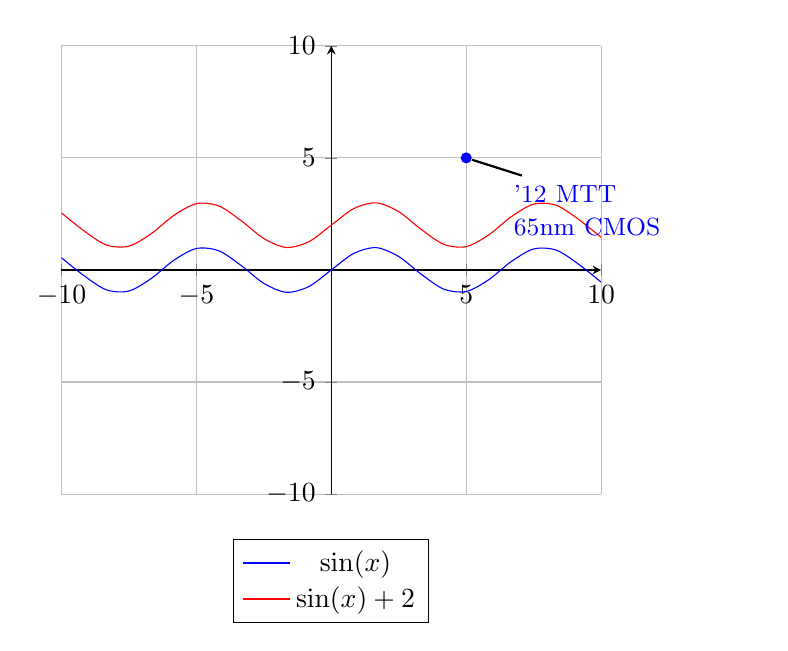
\begin{tikzpicture}
			\begin{axis} [
				axis lines = center,
				xmax = 10,
				xmin = -10,
				ymax = 10,
				ymin = -10,
				grid = major,
				legend style={at={(0.5,-0.1)},anchor=north}
			]
				\addplot[smooth, no marks, blue, domain = -10:10] {sin(deg(x))};
				\addlegendentry{$\sin(x)$}
				\addplot[smooth, no marks, red, domain = -10:10] {sin(deg(x))+ 2};
				\addlegendentry{$\sin(x)+2$}
			\end{axis}
		\end{tikzpicture}
	\end{center}
	\subsubsection*{Reflections}
	\begin{center}
		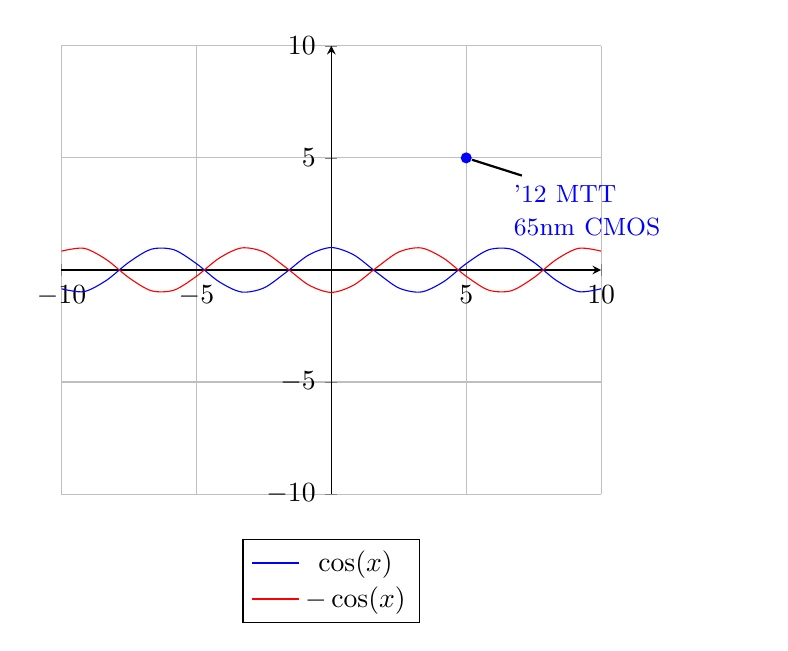
\begin{tikzpicture}
			\begin{axis} [
				axis lines = center,
				xmax = 10,
				xmin = -10,
				ymax = 10,
				ymin = -10,
				grid = major,
				legend style={at={(0.5,-0.1)},anchor=north}
			]
				\addplot[smooth, no marks, blue, domain = -10:10] {cos(deg(x))};
				\addlegendentry{$\cos(x)$}
				\addplot[smooth, no marks, red, domain = -10:10] {-cos(deg(x))};
				\addlegendentry{$-\cos(x)$}
			\end{axis}
		\end{tikzpicture}
	\end{center}
	\section{Analytic Trigonometry}
	\subsection{Reciprocal Identities and Quotient Identities}
	\subsubsection*{Reciprocal Identities}
	\begin{enumerate}
		\item $sin\theta = \frac{1}{csc\theta}$
		\item $cos\theta = \frac{1}{sec\theta}$
		\item $tan\theta = \frac{1}{cot\theta}$
		\item $csc\theta = \frac{1}{sin\theta}$
		\item $sec\theta = \frac{1}{cos\theta}$
		\item $cot\theta = \frac{1}{tan\theta}$
	\end{enumerate}
	\subsubsection*{Quotient Identities}
	\begin{enumerate}
		\item $tan\theta = \frac{sin\theta}{cos\theta}$
		\item $cot\theta = \frac{cos\theta}{sin\theta}$
	\end{enumerate}
	\subsection{Pythagorean Identities}
	\begin{enumerate}
		\item $sin^2\theta + cos^2\theta = 1$
		\item $sin^2\theta = 1 - cos^2\theta$
		\item $cos^2\theta = 1 - sin^2\theta$
	\end{enumerate}
	\subsection{Double Angle Identities}
	\begin{enumerate}
		\item $sin2x = 2sinxcosx$
		\item $cos2x = cos^2x - sin^2x$
		\item $cos2x = 2cos^2x - 1$
		\item $cos2x = 1 - 2sin^2x$
		\item $tan2x = \frac{2 + tanx}{1 - tan^2x}$
	\end{enumerate}
	\subsection{Half Angle Identities}
	\begin{enumerate}
		\item $sin\frac{x}{2} = \pm\sqrt{\frac{1-cosx}{2}}$
		\item $cos\frac{x}{2} = \pm\sqrt{\frac{1+cosx}{2}}$
		\item $tan\frac{x}{2} = \pm\sqrt{\frac{1-cosx}{1+cosx}}$
		\item $tan\frac{x}{2} = \frac{1-cosx}{sinx}$
		\item $tan\frac{x}{2} = \frac{sinx}{1+cosx}$
	\end{enumerate}
	\subsection{Power-Reducing Identities}
	\begin{enumerate}
		\item $sin^2x = \frac{1-cos2x}{2}$
		\item $cos^2x = \frac{1+cos2x}{2}$
		\item $tan^2x = \frac{1-cos2x}{1+cos2x}$
	\end{enumerate}
	\subsection{Simplifying Trig Functions}
	\subsubsection*{Example: $\frac{tan\theta}{sec\theta} = \frac{sin\theta}{cos\theta}$}
	Tip \#1: When possible transform to $sin$ and $cos$. \\
	\\
	$\frac{tan\theta}{sec\theta} = \frac{\frac{sin\theta}{cos\theta}}{\frac{1}{cos\theta}}$ \\
	\\
	$\frac{sin\theta}{\cancel{cos\theta}} * \frac{\cancel{cos\theta}}{1}$ \\
	\\
	$\frac{sin\theta}{1} \to sin\theta$
	\subsubsection*{Example: $\frac{cosx}{1-sinx} - \frac{sinx}{cosx}$}
	Tip \#2: Get a common denominator. \\
	\\
	$\frac{cos^2x-sinx+sin^2x}{(1-sinx)cosx}$ \\
	\\
	$\frac{\cancel{1-sinx}}{\cancel{(1-sinx)}cosx} \to \frac{1}{cosx} = secx$
	\subsubsection*{Example: $sin^3x+sinxcos^2x$}
	Tip \#3: Where there's two terms with something in common, factor it out.\\
	\\
	$sinx(\cancel{sin^2x+cos^2x}) \to sinx$
	\subsection{Solving Trig Equations}
	\subsubsection*{Example: $cos^3x-cosx = 0$}
	$cosx(-sin^2x-1) = 0$ \\
	\\
	$cosx(-sin^2x) = 0$ \\
	\\
	$cosx = 0$ \\
	\\
	$x = \frac{\pi}{2}, \frac{3\pi}{2}$
	\subsubsection*{Example: $5sin^2x+12sinx + 7 = 0$}
	$5x^2+12x+7 = 0$ \\
	\\
	$(5x+7)(x + 1) = 0$ \\
	\\
	$5x + 7=0 \quad x+1=0$ \\
	\\
	$5x + 7 = 0$ \\
	\\
	$sinx = -1$ \\
	\\
	$x = \frac{3\pi}{2}$
	\subsection{Proving Trig Identities}
	\begin{proof}
		\begin{align*}
			tanx + cotx &= secxcscx \\
			\frac{sinx}{cosx} + \frac{cosx}{sinx} &= \\
			\frac{sin^2x+cos^2x}{sinxcosx} &= \\
			\frac{1}{sinxcosx} &= \\
			secxcscx &= &&\qedhere
		\end{align*}
	\end{proof}
	\begin{proof}
		\begin{align*}
			\frac{1}{secx-1} + \frac{1}{secx+1} &= 2cotxcscx \\
			\frac{(secx\cancel{+1}) + (secx\cancel{-1})}{(secx - 1)(secx + 1)} &= \\
			\frac{2secx}{sec^2x-1} &= \\
			\frac{2secx}{tan^x} &= \\
			\frac{\frac{2}{cosx}}{\frac{sin^2x}{cos^2x}} &= \\
			\frac{2}{\cancel{cosx}} \cdot \frac{\cancel{cos^x}}{sin^x} \to \frac{2cosx}{sin^x} &= \\
			\frac{2cosx}{sinx} \cdot \frac{1}{sinx} &= \\
			2cotxcscx &= &&\qedhere
		\end{align*}
	\end{proof}
	\subsection{Law of Sines}
	Finding missing side lengths and angle measurements in non-right $\Delta$s \\
	\vspace{5mm}
	\begin{center}
		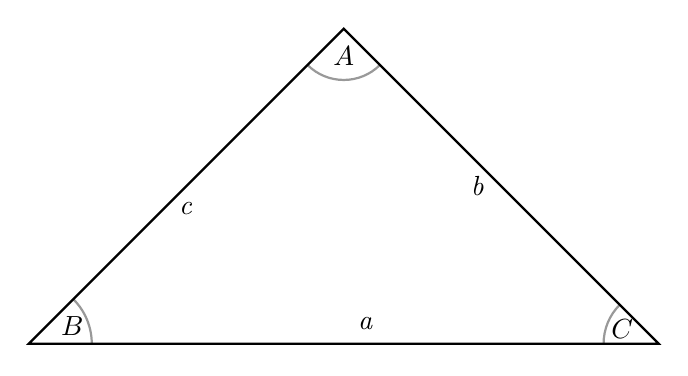
\begin{tikzpicture}[thick]
			\coordinate (O) at (4,4);
			\coordinate (A) at (0,0);
			\coordinate (B) at (8,0);
			\draw (O)--(A)--(B)--cycle;
			
			\tkzLabelSegment[below=2pt](O,A){\textit{c}}
			\tkzLabelSegment[left=2pt](O,B){\textit{b}}
			\tkzLabelSegment[above right=2pt](A,B){\textit{a}}
			
			\tkzMarkAngle[fill= orange,size=0.65cm,%
			opacity=.4](A,O,B)
			\tkzLabelAngle[pos = 0.35](A,O,B){$A$}
			
			\tkzMarkAngle[fill= orange,size=0.8cm,%
			opacity=.4](B,A,O)
			\tkzLabelAngle[pos = 0.6](B,A,O){$B$}
			
			\tkzMarkAngle[fill= orange,size=0.7cm,%
			opacity=.4](O,B,A)
			\tkzLabelAngle[pos = 0.5](O,B,A){$C$}
		\end{tikzpicture}
		\\
		$\frac{sinA}{a} = \frac{sinB}{b} = \frac{sinC}{c}$
		\\
		\subsubsection*{Example: $A = 15\degree \;C = 109\degree \;c = 46$ find a, B, b}
		$B = 180 - 15 - 109 = 56$ \\
		$\frac{sin15}{a} = \frac{sin109}{46}$ \\
		$11.91 = a(0.95) \to a = 12.59$ \\
		$\frac{sin56}{b} = \frac{sin109}{46} \to b = 40.33$ \\
		\subsubsection*{Example: $a = 7 \;b = 6 \;A = 26.3\degree$ find B, C, c}
		$\frac{sin26.3}{7} = \frac{sinB}{6}$ \\
		$0.36 = sinB$ \\
		$B = 22.3\degree$ \\
		$180 - 22.3 = 131.4\degree$ \\
		$C = 131.4\degree$ \\
		$c = 11.85$ \\
	\end{center}
	\subsection{Law of Cosines}
	\begin{enumerate}
		\item $a^2 = b^2 + c^2 - 2bccosA$
		\item $b^2 = a^2 + c^2 - 2accosB$
		\item $c^2 = a^2 + b^2 - 2abcosC$
	\end{enumerate}
	\subsubsection*{Example: $a = 7 \; c = 5 \; B = 97.3\degree$}
	$b^2 = 7^2 + 5^2 - 2(7)(5)cos(97.3)$ \\
	\\
	$\sqrt{b^2} = \sqrt{82.89\degree}$ \\
	\\
	$b = 9.1\degree$ \\
	\\
	$25 = 49 + 82.81 - 2(7)(9.1)cosC$ \\
	\\
	$25 = 49 + 82.8 - 127.4cosC$ \\
	\\
	$25 = 131.81 - 127.4cosC$ \\
	\\
	$\frac{-106.81}{-127.4} = \frac{-127.4cosC}{-127.4}$ \\
	\\
	$A = 119.6$ \\
	\\
	$(0.838)^{-1} = {cosC}^{-1}$ \\
	\\
	$33.1\degree = C$
	\subsection{Area of a Triangle (SAS and SSS)}
	\subsubsection*{SAS: $\frac{1}{2}absinC$}
	\begin{center}
		\begin{tikzpicture}[thick]
			\coordinate (O) at (4,4);
			\coordinate (A) at (0,0);
			\coordinate (B) at (8,-4);
			\draw (O)--(A)--(B)--cycle;
			
			\tkzLabelSegment[below=2pt](O,A){\textit{}}
			\tkzLabelSegment[left=2pt](O,B){\textit{16}}
			\tkzLabelSegment[above right=2pt](A,B){\textit{4}}
			
			\tkzMarkAngle[fill= orange,size=0.65cm,%
			opacity=.4](A,O,B)
			\tkzLabelAngle[pos = 0.35](A,O,B){}
			
			\tkzMarkAngle[fill= orange,size=0.8cm,%
			opacity=.4](B,A,O)
			\tkzLabelAngle[pos = 0.6](B,A,O){}
			
			\tkzMarkAngle[fill= orange,size=0.7cm,%
			opacity=.4](O,B,A)
			\tkzLabelAngle[pos = 1](O,B,A){$36\degree$}
		\end{tikzpicture}
		\\
		$A = \frac{1}{2}(4)(16)sin36$ \\
		$A = 18.81\; units^2$
	\end{center}
	\subsubsection*{SSS: Heron's Formula: $A = \sqrt{(s)(s-a)(s-b)(s-c)}$}
	\begin{center}
		\begin{tikzpicture}[thick]
			\coordinate (O) at (4,4);
			\coordinate (A) at (0,0);
			\coordinate (B) at (8,-4);
			\draw (O)--(A)--(B)--cycle;
			
			\tkzLabelSegment[below=2pt](O,A){\textit{17}}
			\tkzLabelSegment[left=2pt](O,B){\textit{41}}
			\tkzLabelSegment[above right=2pt](A,B){\textit{38}}
			
			\tkzMarkAngle[fill= orange,size=0.65cm,%
			opacity=.4](A,O,B)
			\tkzLabelAngle[pos = 0.35](A,O,B){}
			
			\tkzMarkAngle[fill= orange,size=0.8cm,%
			opacity=.4](B,A,O)
			\tkzLabelAngle[pos = 0.6](B,A,O){}
			
			\tkzMarkAngle[fill= orange,size=0.7cm,%
			opacity=.4](O,B,A)
			\tkzLabelAngle[pos = 1](O,B,A){}
		\end{tikzpicture}
		\\
		$s = 48$ \\
		$A = \sqrt{(48)(48-17)(48-38)(48-41)}$ \\
		$A = 322.738\; units^2$
	\end{center}
\end{document}